\chapter{АРХИТЕКТУРА И ПРОЕКТИРОВАНИЕ СИСТЕМЫ РЕКОМЕНДАЦИИ НОВОСТЕЙ}

В данной главе рассматривается архитектура и проектирование разрабатываемой системы рекомендации новостей. Описание основных компонентов и модулей, входящих в состав системы, и взаимодействия между ними.

\section{Формулирование требований к системе рекомендации новостей}
Исходя из целей работы и проведенного аналитического обзора, была поставлена задача разработать бота для Telegram, позволяющего получать персонализированные рекомендации новостей, краткий пересказ интересующих новостей и групповых чатов, отвечать на вопросы с использованием информации из новостей и групповых чатов в интерактивном режиме.

Были сформулированы следующие требования к разрабатываемой системе:
\begin{enumerate}
    \item чат-бот должен предоставлять пользователю возможность настраивать личные предпочтения путем пересылки интересующих и не интересующих новостей и сообщений из каналов и групповых чатов;
    \item чат-бот должен предоставлять ежедневный и/или еженедельный отчёт с кратким пересказом основной интересующей информации из указанных каналов и групповых чатов;
    \item чат-бот должен предоставлять оригиналы интересующих новостей и сообщений из групповых чатов;
    \item чат-бот должен иметь возможность работать в диалоговом режиме, отвечая на вопросы по содержанию новостей и/или групповых чатов.
\end{enumerate}

\section{Проектирование архитектуры системы}

На основе сфомулированных требований к системе и анализа предметной области, была разработана архитектура системы, представленная на рисунке \ref{img:system_architecture}. Она основана на работе \cite{news_rec_gen}.

\begin{figure}[h]
    \centering
    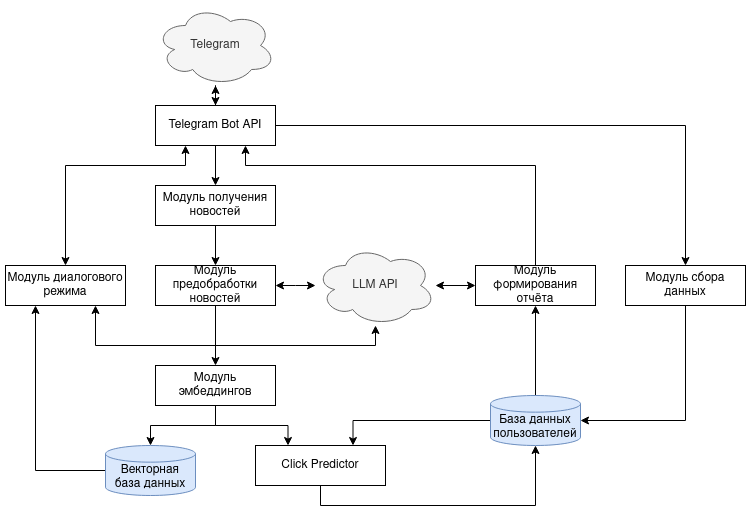
\includegraphics[width=\linewidth]{../images/system_architecture.drawio.png}
    \caption{Архитектура системы}
    \label{img:system_architecture}
\end{figure}

Основные компоненты системы
\begin{enumerate}
    \item Telegram Bot API ~-- фасад системы, реализующий взаимодействие с ней с помощью чат-бота в Telegram;
    \item модуль получения новостей осуществляет загрузку новостей из каналов, на которые подписаны пользователи;
    \item модуль предобработки новостей осуществляет предобработку и обогощение данных с помощью большой языковой модели, как представлено в рааботе \cite{news_rec_gen};
    \item модуль эмбеддингов формирует векторное представление новостей;
    \item модуль Click Predictor осуществляет бинарную классификацию будет ли новость показана тому или иному пользователию или нет;
    \item модуль формирования отчёта собирает рекомендованные для  пользователя новости и формирует краткий пересказ;
    \item модуль сбора данных получает обратную связь от пользователя для определения его предпочтений и настройки рекомендательной системы;
    \item модуль диалогового режима осуществляет интерактивное взаимодействие с пользователем на с помощью большой языковой модели.
    \item векторная база данных хранит новости и их векторные представления;
    \item база данных пользователей хранит пользователей, их историю просмотра новостей, их настройки предпочтений, векторное представление пользователей и список рекомендованных новостей.
\end{enumerate}

Система работает следующим образом. Первоначально, каждый пользователь настраивает свои предпочтения, отправляя чат-боту новости, которые он хочет и не хочет видеть в своих рекомендациях. Эти новости проходят через процесс обработки и векторизации и на их основе формируются эмбеддинги пользоваталей, сохраняемые в базе данных.

Система работает в событийно-ориентированном режиме, обрабатывая новости, публикуемые в отслеживаемых каналах:
\begin{enumerate}
    \item новости загружаются модулем получения новостей;
    \item затем осуществляется предобработка новостей, включающая в себя сумморизацию новости с помощью большой языковой модели;
    \item на основе данных новости и сумморизированного текста новости формируется векторное представление новости, которое сохраняется в базе данных для дальнейшего использования;
    \item модуль click precictor осуществляет классификацию: нужно ли показывать новость пользователю или нет;
    \item в зависимости от настроек, рекомендованная новсть может быть показана пользователю, либо сохранена в базе данных пользователей для дальнейшего формирования отчёта;
\end{enumerate}

С заданным интервалом запускается модуль формирования отчёта, который извлекает рекомендуемые новости за указанный период из базы данных, сумморизирует их с использованием большой языковой модели, и отправляет пользователию.

При работе с системой в диалоговом режиме, используется большая языковая модель. Чтобы реализовать работу с собранными данными новостей, LLM взаимодействует с векторной базой данных новостей, которая используется как внешнее хранилище. Нужные новости извлекаются из базы и подставляются в контекст языковой модели.

Для работы модуля эмбеддингов применяется запущенная локально языковая модель BERT или LLaMA. Для работы модулей сумморизации и диалогового режима применяется закрытая большая языковая модель, доступная в качестве сервиса, такие как ChatGPT или YandexGPT.
